% LIMIT on-demand concept trial. Generated by build_limit_trial.py.
% Not included by the paper. Not a measured result. Not an execution trace.
\documentclass{article}
\usepackage[T1]{fontenc}
\usepackage{mathptmx}
\usepackage{tikz}
\usetikzlibrary{arrows.meta}
\pagestyle{empty}
\setlength{\paperwidth}{178.00mm}
\setlength{\paperheight}{87.75mm}
\pdfpagewidth=\paperwidth
\pdfpageheight=\paperheight
\setlength{\hoffset}{-1in}
\setlength{\voffset}{-1in}
\setlength{\oddsidemargin}{0pt}
\setlength{\topmargin}{0pt}
\setlength{\headheight}{0pt}
\setlength{\headsep}{0pt}
\setlength{\topskip}{0pt}
\setlength{\footskip}{0pt}
\setlength{\marginparsep}{0pt}
\setlength{\marginparwidth}{0pt}
\setlength{\textwidth}{\paperwidth}
\setlength{\textheight}{\paperheight}
\setlength{\parindent}{0pt}
\definecolor{ink}{HTML}{262B30}
\definecolor{yieldblue}{HTML}{1F6F8B}
\definecolor{bluefill}{HTML}{E5F1F7}
\definecolor{muted}{HTML}{5C6B76}
\definecolor{aclgray}{HTML}{8E99A4}
\definecolor{rule}{HTML}{C5CED4}
\begin{document}%
\nointerlineskip
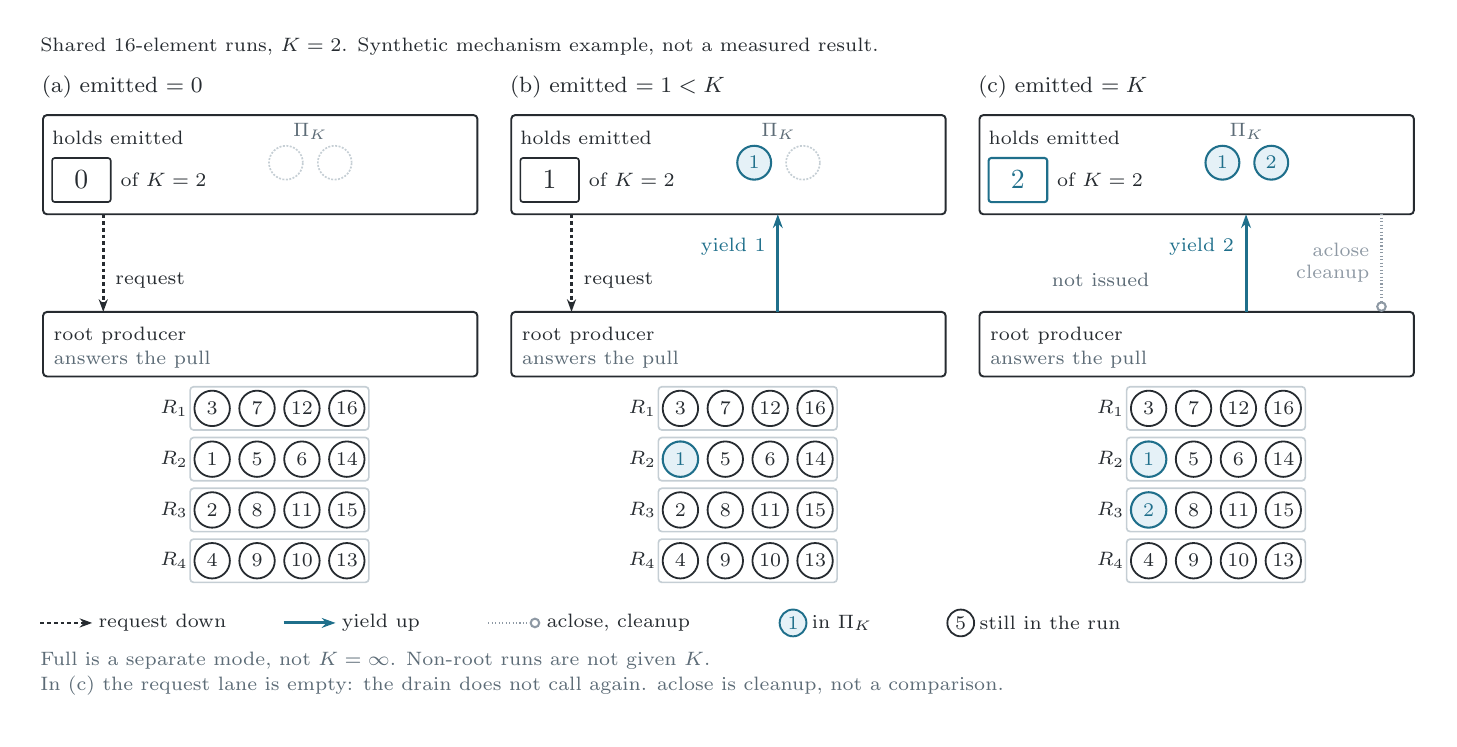
\begin{tikzpicture}[x=1mm,y=1mm,
  every node/.style={inner sep=0pt, outer sep=0pt},
  box/.style={draw=ink, line width=0.7pt, rounded corners=0.5mm},
  runbox/.style={draw=rule, line width=0.6pt, rounded corners=0.45mm},
  counter/.style={draw=ink, line width=0.6pt, rounded corners=0.35mm, fill=white},
  countermet/.style={counter, draw=yieldblue, line width=0.75pt},
  req/.style={draw=ink, line width=0.9pt, dash pattern=on 1.4pt off 1.05pt,
    -{Stealth[length=1.6mm,width=1.15mm]}},
  yld/.style={draw=yieldblue, line width=1.05pt,
    -{Stealth[length=1.75mm,width=1.25mm]}},
  acl/.style={draw=aclgray, line width=0.75pt, dash pattern=on 0.4pt off 0.85pt,
    -{Circle[open,length=1.35mm]}},
  fsmall/.style={font=\fontsize{6.6}{7.4}\selectfont},
  ftitle/.style={font=\fontsize{8}{9}\selectfont},
  fnum/.style={font=\fontsize{7}{8}\selectfont},
  fcount/.style={font=\fontsize{10}{11}\selectfont}
]
\useasboundingbox (0,0) rectangle (178.00,87.75);
\node[anchor=west, fsmall, text=ink] at (1.6,85.35) {Shared 16-element runs, $K=2$. Synthetic mechanism example, not a measured result.};
\draw[req] (1.6,12.15) -- (8.2,12.15);
\node[anchor=west, fsmall, text=ink] at (9.0,12.15) {request down};
\draw[yld] (32.5,12.15) -- (39.1,12.15);
\node[anchor=west, fsmall, text=ink] at (39.9,12.15) {yield up};
\draw[acl] (58.5,12.15) -- (65.1,12.15);
\node[anchor=west, fsmall, text=ink] at (65.9,12.15) {aclose, cleanup};
\draw[fill=bluefill, draw=yieldblue, line width=0.7pt] (97.2,12.15) circle (1.7);
\node[fnum, text=yieldblue] at (97.2,12.15) {1};
\node[anchor=west, fsmall, text=ink] at (99.6,12.15) {in $\Pi_K$};
\draw[fill=white, draw=ink, line width=0.65pt] (118.5,12.15) circle (1.7);
\node[fnum, text=ink] at (118.5,12.15) {5};
\node[anchor=west, fsmall, text=ink] at (120.9,12.15) {still in the run};
\node[anchor=west, fsmall, text=muted] at (1.6,7.35) {Full is a separate mode, not $K=\infty$. Non-root runs are not given $K$.};
\node[anchor=west, fsmall, text=muted] at (1.6,4.15) {In (c) the request lane is empty: the drain does not call again. aclose is cleanup, not a comparison.};
\begin{scope}[shift={(1.400,16.800)}]
\node[anchor=west, ftitle, text=ink] at (0.4,63.45) {(a) emitted $= 0$};
\draw[box] (0.55,47.25) rectangle (55.72,59.85);
\draw[box] (0.55,26.65) rectangle (55.72,34.85);
\draw[counter] (1.70,48.80) rectangle (9.15,54.40);
\node[fcount, text=ink] at (5.42,51.60) {0};
\node[anchor=west, fsmall, text=ink] at (1.70,57.00) {holds emitted};
\node[anchor=west, fsmall, text=ink] at (10.40,51.60) {of $K=2$};
\node[anchor=center, fsmall, text=muted] at (34.50,57.80) {$\Pi_K$};
\draw[fill=white, draw=rule, line width=0.6pt, dash pattern=on 0.7pt off 0.55pt] (31.40,53.80) circle (2.15);
\draw[fill=white, draw=rule, line width=0.6pt, dash pattern=on 0.7pt off 0.55pt] (37.60,53.80) circle (2.15);
\node[anchor=west, fsmall, text=ink] at (1.90,31.80) {root producer};
\node[anchor=west, fsmall, text=muted] at (1.90,28.80) {answers the pull};
\draw[runbox] (19.23,19.85) rectangle (41.93,25.35);
\node[anchor=east, fnum, text=ink] at (18.93,22.60) {$R_1$};
\draw[fill=white, draw=ink, line width=0.65pt] (22.03,22.60) circle (2.25);
\node[fnum, text=ink] at (22.03,22.60) {3};
\draw[fill=white, draw=ink, line width=0.65pt] (27.73,22.60) circle (2.25);
\node[fnum, text=ink] at (27.73,22.60) {7};
\draw[fill=white, draw=ink, line width=0.65pt] (33.43,22.60) circle (2.25);
\node[fnum, text=ink] at (33.43,22.60) {12};
\draw[fill=white, draw=ink, line width=0.65pt] (39.13,22.60) circle (2.25);
\node[fnum, text=ink] at (39.13,22.60) {16};
\draw[runbox] (19.23,13.40) rectangle (41.93,18.90);
\node[anchor=east, fnum, text=ink] at (18.93,16.15) {$R_2$};
\draw[fill=white, draw=ink, line width=0.65pt] (22.03,16.15) circle (2.25);
\node[fnum, text=ink] at (22.03,16.15) {1};
\draw[fill=white, draw=ink, line width=0.65pt] (27.73,16.15) circle (2.25);
\node[fnum, text=ink] at (27.73,16.15) {5};
\draw[fill=white, draw=ink, line width=0.65pt] (33.43,16.15) circle (2.25);
\node[fnum, text=ink] at (33.43,16.15) {6};
\draw[fill=white, draw=ink, line width=0.65pt] (39.13,16.15) circle (2.25);
\node[fnum, text=ink] at (39.13,16.15) {14};
\draw[runbox] (19.23,6.95) rectangle (41.93,12.45);
\node[anchor=east, fnum, text=ink] at (18.93,9.70) {$R_3$};
\draw[fill=white, draw=ink, line width=0.65pt] (22.03,9.70) circle (2.25);
\node[fnum, text=ink] at (22.03,9.70) {2};
\draw[fill=white, draw=ink, line width=0.65pt] (27.73,9.70) circle (2.25);
\node[fnum, text=ink] at (27.73,9.70) {8};
\draw[fill=white, draw=ink, line width=0.65pt] (33.43,9.70) circle (2.25);
\node[fnum, text=ink] at (33.43,9.70) {11};
\draw[fill=white, draw=ink, line width=0.65pt] (39.13,9.70) circle (2.25);
\node[fnum, text=ink] at (39.13,9.70) {15};
\draw[runbox] (19.23,0.50) rectangle (41.93,6.00);
\node[anchor=east, fnum, text=ink] at (18.93,3.25) {$R_4$};
\draw[fill=white, draw=ink, line width=0.65pt] (22.03,3.25) circle (2.25);
\node[fnum, text=ink] at (22.03,3.25) {4};
\draw[fill=white, draw=ink, line width=0.65pt] (27.73,3.25) circle (2.25);
\node[fnum, text=ink] at (27.73,3.25) {9};
\draw[fill=white, draw=ink, line width=0.65pt] (33.43,3.25) circle (2.25);
\node[fnum, text=ink] at (33.43,3.25) {10};
\draw[fill=white, draw=ink, line width=0.65pt] (39.13,3.25) circle (2.25);
\node[fnum, text=ink] at (39.13,3.25) {13};
\draw[req] (8.20,47.25) -- (8.20,34.85);
\node[anchor=west, fsmall, text=ink] at (9.75,38.90) {request};
\end{scope}
\begin{scope}[shift={(60.867,16.800)}]
\node[anchor=west, ftitle, text=ink] at (0.4,63.45) {(b) emitted $= 1 < K$};
\draw[box] (0.55,47.25) rectangle (55.72,59.85);
\draw[box] (0.55,26.65) rectangle (55.72,34.85);
\draw[counter] (1.70,48.80) rectangle (9.15,54.40);
\node[fcount, text=ink] at (5.42,51.60) {1};
\node[anchor=west, fsmall, text=ink] at (1.70,57.00) {holds emitted};
\node[anchor=west, fsmall, text=ink] at (10.40,51.60) {of $K=2$};
\node[anchor=center, fsmall, text=muted] at (34.50,57.80) {$\Pi_K$};
\draw[fill=bluefill, draw=yieldblue, line width=0.75pt] (31.40,53.80) circle (2.15);
\node[fnum, text=yieldblue] at (31.40,53.80) {1};
\draw[fill=white, draw=rule, line width=0.6pt, dash pattern=on 0.7pt off 0.55pt] (37.60,53.80) circle (2.15);
\node[anchor=west, fsmall, text=ink] at (1.90,31.80) {root producer};
\node[anchor=west, fsmall, text=muted] at (1.90,28.80) {answers the pull};
\draw[runbox] (19.23,19.85) rectangle (41.93,25.35);
\node[anchor=east, fnum, text=ink] at (18.93,22.60) {$R_1$};
\draw[fill=white, draw=ink, line width=0.65pt] (22.03,22.60) circle (2.25);
\node[fnum, text=ink] at (22.03,22.60) {3};
\draw[fill=white, draw=ink, line width=0.65pt] (27.73,22.60) circle (2.25);
\node[fnum, text=ink] at (27.73,22.60) {7};
\draw[fill=white, draw=ink, line width=0.65pt] (33.43,22.60) circle (2.25);
\node[fnum, text=ink] at (33.43,22.60) {12};
\draw[fill=white, draw=ink, line width=0.65pt] (39.13,22.60) circle (2.25);
\node[fnum, text=ink] at (39.13,22.60) {16};
\draw[runbox] (19.23,13.40) rectangle (41.93,18.90);
\node[anchor=east, fnum, text=ink] at (18.93,16.15) {$R_2$};
\draw[fill=bluefill, draw=yieldblue, line width=0.75pt] (22.03,16.15) circle (2.25);
\node[fnum, text=yieldblue] at (22.03,16.15) {1};
\draw[fill=white, draw=ink, line width=0.65pt] (27.73,16.15) circle (2.25);
\node[fnum, text=ink] at (27.73,16.15) {5};
\draw[fill=white, draw=ink, line width=0.65pt] (33.43,16.15) circle (2.25);
\node[fnum, text=ink] at (33.43,16.15) {6};
\draw[fill=white, draw=ink, line width=0.65pt] (39.13,16.15) circle (2.25);
\node[fnum, text=ink] at (39.13,16.15) {14};
\draw[runbox] (19.23,6.95) rectangle (41.93,12.45);
\node[anchor=east, fnum, text=ink] at (18.93,9.70) {$R_3$};
\draw[fill=white, draw=ink, line width=0.65pt] (22.03,9.70) circle (2.25);
\node[fnum, text=ink] at (22.03,9.70) {2};
\draw[fill=white, draw=ink, line width=0.65pt] (27.73,9.70) circle (2.25);
\node[fnum, text=ink] at (27.73,9.70) {8};
\draw[fill=white, draw=ink, line width=0.65pt] (33.43,9.70) circle (2.25);
\node[fnum, text=ink] at (33.43,9.70) {11};
\draw[fill=white, draw=ink, line width=0.65pt] (39.13,9.70) circle (2.25);
\node[fnum, text=ink] at (39.13,9.70) {15};
\draw[runbox] (19.23,0.50) rectangle (41.93,6.00);
\node[anchor=east, fnum, text=ink] at (18.93,3.25) {$R_4$};
\draw[fill=white, draw=ink, line width=0.65pt] (22.03,3.25) circle (2.25);
\node[fnum, text=ink] at (22.03,3.25) {4};
\draw[fill=white, draw=ink, line width=0.65pt] (27.73,3.25) circle (2.25);
\node[fnum, text=ink] at (27.73,3.25) {9};
\draw[fill=white, draw=ink, line width=0.65pt] (33.43,3.25) circle (2.25);
\node[fnum, text=ink] at (33.43,3.25) {10};
\draw[fill=white, draw=ink, line width=0.65pt] (39.13,3.25) circle (2.25);
\node[fnum, text=ink] at (39.13,3.25) {13};
\draw[req] (8.20,47.25) -- (8.20,34.85);
\node[anchor=west, fsmall, text=ink] at (9.75,38.90) {request};
\draw[yld] (34.40,34.85) -- (34.40,47.25);
\node[anchor=east, fsmall, text=yieldblue] at (32.85,43.20) {yield 1};
\end{scope}
\begin{scope}[shift={(120.333,16.800)}]
\node[anchor=west, ftitle, text=ink] at (0.4,63.45) {(c) emitted $= K$};
\draw[box] (0.55,47.25) rectangle (55.72,59.85);
\draw[box] (0.55,26.65) rectangle (55.72,34.85);
\draw[countermet] (1.70,48.80) rectangle (9.15,54.40);
\node[fcount, text=yieldblue] at (5.42,51.60) {2};
\node[anchor=west, fsmall, text=ink] at (1.70,57.00) {holds emitted};
\node[anchor=west, fsmall, text=ink] at (10.40,51.60) {of $K=2$};
\node[anchor=center, fsmall, text=muted] at (34.50,57.80) {$\Pi_K$};
\draw[fill=bluefill, draw=yieldblue, line width=0.75pt] (31.40,53.80) circle (2.15);
\node[fnum, text=yieldblue] at (31.40,53.80) {1};
\draw[fill=bluefill, draw=yieldblue, line width=0.75pt] (37.60,53.80) circle (2.15);
\node[fnum, text=yieldblue] at (37.60,53.80) {2};
\node[anchor=west, fsmall, text=ink] at (1.90,31.80) {root producer};
\node[anchor=west, fsmall, text=muted] at (1.90,28.80) {answers the pull};
\draw[runbox] (19.23,19.85) rectangle (41.93,25.35);
\node[anchor=east, fnum, text=ink] at (18.93,22.60) {$R_1$};
\draw[fill=white, draw=ink, line width=0.65pt] (22.03,22.60) circle (2.25);
\node[fnum, text=ink] at (22.03,22.60) {3};
\draw[fill=white, draw=ink, line width=0.65pt] (27.73,22.60) circle (2.25);
\node[fnum, text=ink] at (27.73,22.60) {7};
\draw[fill=white, draw=ink, line width=0.65pt] (33.43,22.60) circle (2.25);
\node[fnum, text=ink] at (33.43,22.60) {12};
\draw[fill=white, draw=ink, line width=0.65pt] (39.13,22.60) circle (2.25);
\node[fnum, text=ink] at (39.13,22.60) {16};
\draw[runbox] (19.23,13.40) rectangle (41.93,18.90);
\node[anchor=east, fnum, text=ink] at (18.93,16.15) {$R_2$};
\draw[fill=bluefill, draw=yieldblue, line width=0.75pt] (22.03,16.15) circle (2.25);
\node[fnum, text=yieldblue] at (22.03,16.15) {1};
\draw[fill=white, draw=ink, line width=0.65pt] (27.73,16.15) circle (2.25);
\node[fnum, text=ink] at (27.73,16.15) {5};
\draw[fill=white, draw=ink, line width=0.65pt] (33.43,16.15) circle (2.25);
\node[fnum, text=ink] at (33.43,16.15) {6};
\draw[fill=white, draw=ink, line width=0.65pt] (39.13,16.15) circle (2.25);
\node[fnum, text=ink] at (39.13,16.15) {14};
\draw[runbox] (19.23,6.95) rectangle (41.93,12.45);
\node[anchor=east, fnum, text=ink] at (18.93,9.70) {$R_3$};
\draw[fill=bluefill, draw=yieldblue, line width=0.75pt] (22.03,9.70) circle (2.25);
\node[fnum, text=yieldblue] at (22.03,9.70) {2};
\draw[fill=white, draw=ink, line width=0.65pt] (27.73,9.70) circle (2.25);
\node[fnum, text=ink] at (27.73,9.70) {8};
\draw[fill=white, draw=ink, line width=0.65pt] (33.43,9.70) circle (2.25);
\node[fnum, text=ink] at (33.43,9.70) {11};
\draw[fill=white, draw=ink, line width=0.65pt] (39.13,9.70) circle (2.25);
\node[fnum, text=ink] at (39.13,9.70) {15};
\draw[runbox] (19.23,0.50) rectangle (41.93,6.00);
\node[anchor=east, fnum, text=ink] at (18.93,3.25) {$R_4$};
\draw[fill=white, draw=ink, line width=0.65pt] (22.03,3.25) circle (2.25);
\node[fnum, text=ink] at (22.03,3.25) {4};
\draw[fill=white, draw=ink, line width=0.65pt] (27.73,3.25) circle (2.25);
\node[fnum, text=ink] at (27.73,3.25) {9};
\draw[fill=white, draw=ink, line width=0.65pt] (33.43,3.25) circle (2.25);
\node[fnum, text=ink] at (33.43,3.25) {10};
\draw[fill=white, draw=ink, line width=0.65pt] (39.13,3.25) circle (2.25);
\node[fnum, text=ink] at (39.13,3.25) {13};
\node[anchor=west, fsmall, text=muted] at (9.75,38.90) {not issued};
\draw[yld] (34.40,34.85) -- (34.40,47.25);
\node[anchor=east, fsmall, text=yieldblue] at (32.85,43.20) {yield 2};
\draw[acl] (51.60,47.25) -- (51.60,34.85);
\node[anchor=east, fsmall, text=aclgray] at (50.05,42.75) {aclose};
\node[anchor=east, fsmall, text=aclgray] at (50.05,39.70) {cleanup};
\end{scope}
\end{tikzpicture}%
\end{document}
